%Valid Execution Rules---------------------------------------------------------------------------------------------------------------------------------
        
    \section{Valid Execution Rules (the Axioms)}
        We now state the memory consistency rules. The rules are on \textit{Candidate Executions} which will place constraints on the possible \textit{Observable behaviors} that may result from it. 
         
%--------------------------------------------------------------------------------------------------------------------------------------  
        %Coherent Reads   
        \begin{axiom}{Coherent Reads} 
            \label{CoRe}
        
            There are certain restrictions of what a read event cannot see at different points of execution based on $\stck{_{hb}}$ relation with write events. 

            Consider a read event $e$ and a write event $d$ having at least overlapping ranges:
            \begin{align*}
                \event{e}{R} \ \wedge \ 
                \event{d}{W} \ \wedge \
                (\Re(e) \cap_\Re \Re(d) \neq \phi).
            \end{align*}

            \begin{itemize}
                %Rule #1
                \item A read value cannot come from a write that has happened after it 
                    \begin{align*}
                        \reln{e}{hb}{d}\ \Rightarrow{}\ \neg \ \reln{e}{rf}{d}.
                    \end{align*}
                    Figure~\ref{model:coherent_reads(1)} pictorially depicts the pattern above hwere $e$ cannot read from $d$.
                    \begin{figure}[H]
                        \centering
                        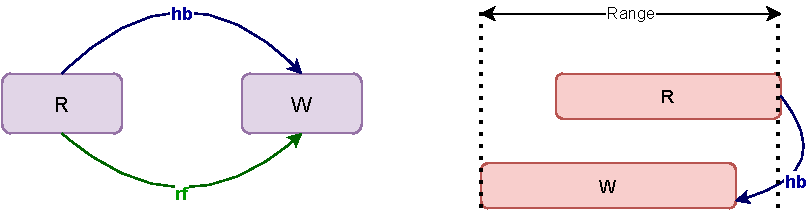
\includegraphics[scale=0.7]{4.ECMAScriptMemoryModel/CoherentReads1.pdf}
                        \caption{First axiom of Coherent Reads.}
                        \label{model:coherent_reads(1)}
                    \end{figure}
                %Rule #2    
                \item A read cannot read a specific byte address value from write if there is a write $g$ that happens between them which modifies the exact byte address. Note that this rule would be on the $rbf$ relation among two events. 
                    \begin{align*}
                        \reln{d}{hb}{e}
                        \ \wedge \ 
                        \reln{d}{hb}{g} \ \wedge \  \reln{g}{hb}{e}
                        \ \Rightarrow{} \
                        \forall x \in (\Re(d) \cap_\Re \Re(g) \cap_\Re \Re(e)), \ \neg \ \reln{e}{rbf}{(d,x)}.
                    \end{align*}
                    Figure~\ref{model:coherent_reads(2)} pictorially depicts the pattern where $e$ cannot read certain bytes from $d$. 
                    \begin{figure}[H]
                        \centering 
                        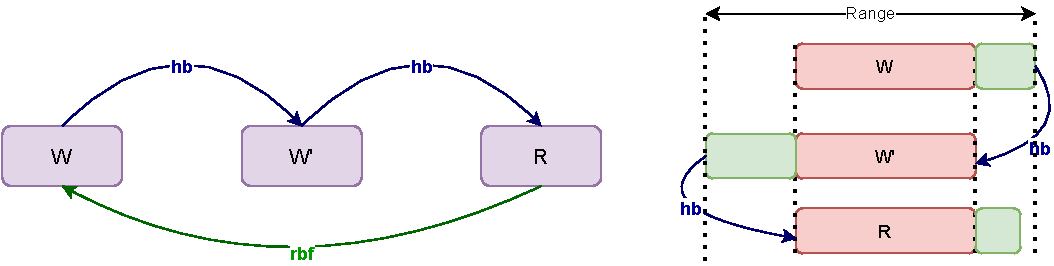
\includegraphics[scale=0.7]{4.ECMAScriptMemoryModel/CoherentReads2.pdf}
                        \caption{Second axiom of Coherent Reads.}
                        \label{model:coherent_reads(2)}
                    \end{figure}
                            
            \end{itemize}
        \end{axiom}
%------------------------------------------------------------------------------------------------------------------------------------------

        \begin{axiom}{Tear-Free Reads} 
            \label{TfRe}

            If two tear free writes $d$ and $g$ and a tear free read $e$ all with equal ranges exist, then $e$ can read only from one of them\footnotemark.
                
            \begin{align*}
                \et{d}{tf}\ \wedge\ \et{g}{tf} \ \wedge \ \et{e}{tf} 
                  \ \wedge \ 
                  (\Re(d) \!=\! \Re(g) \!=\! \Re(e)) 
                  \ \Rightarrow{} \\ 
                      ((\reln{e}{rf}{d}) 
                      \ \wedge \ 
                      (\neg \ \reln{e}{rf}{g})) 
                  \ \vee \  
                      ((\reln{e}{rf}{g}) 
                      \ \wedge \
                      (\neg \ \reln{e}{rf}{d})).
            \end{align*}
                    
            Figure~\ref{model:tear_free_reads(1)} shows the pattern that is disallowed among all tear-free events. 
            \begin{figure}[H]
                \centering
                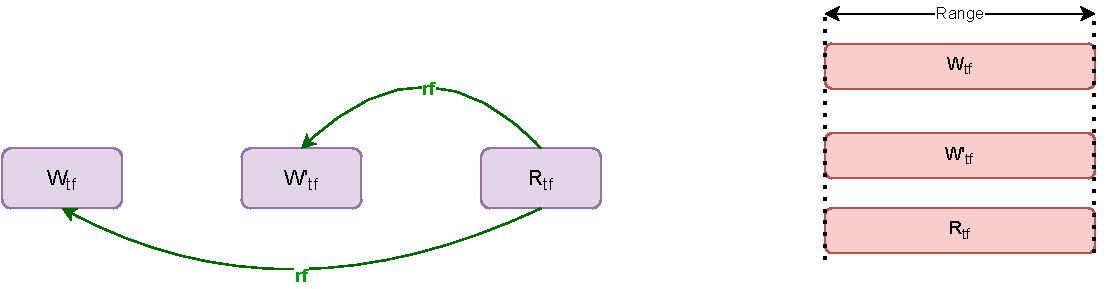
\includegraphics[scale=0.7]{4.ECMAScriptMemoryModel/TearFreeReads.pdf}
                \caption{Axiom of Tear-free reads.}
                \label{model:tear_free_reads}
            \end{figure}

            \footnotetext{To recap a tear-free event cannot be separated into multiple small events that do the same operation. However, considering different hardware architectures, the notion of tear-free need not necessarily mean this. (eg: A 64bit tear-free write to be done in a 32bit system). In a more abstract sense, we need an event to appear 'tear-free'.}    
        \end{axiom}

        \begin{axiom}{Sequentially Consistent Atomics}
            \label{SeqCsAt}   
            
            To specifically define how events that are sequentially consistent affects what values a read cannot see, we assume the following memory order among writes $d$ and $g$ and a read $e$ to be the premise for all the rules:  
                \begin{align*}
                    d \stck{_{mo}} g \stck{_{mo}} e.
                \end{align*}
               
            \begin{itemize}
                \item If all three events are of type $sc$ with equal ranges, then $e$ cannot read from $d$.
                    \begin{align*}
                        \et{d}{sc}\ \wedge\ \et{g}{sc}\ \wedge\ \et{e}{sc} 
                        \ \wedge \ (\Re(d) \!=\! \Re(g) \!=\! \Re(e))
                        \ \Rightarrow{} \ 
                        \neg \ \reln{e}{rf}{d}.
                    \end{align*} 
                        
                    Figure~\ref{model:sc_atomics(1)} depicts pictorially the pattern that is not allowed by this rule.
                    \begin{figure}[H]
                        \centering 
                        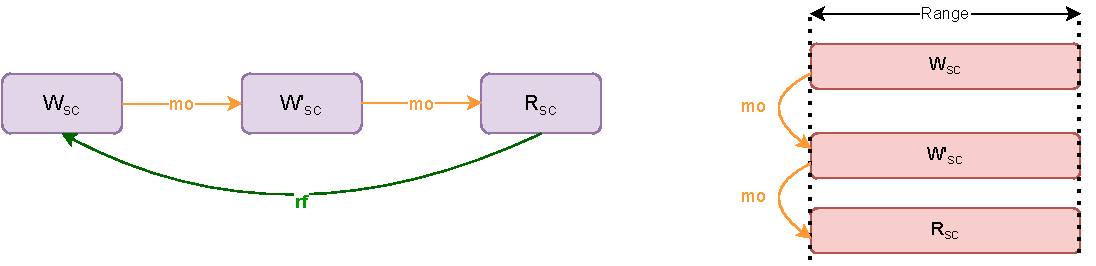
\includegraphics[scale=0.7]{4.ECMAScriptMemoryModel/SequentialAtomics1.pdf}
                        \caption{First Axiom of SC-Atomics.}
                        \label{model:sc_atomics(1)}
                    \end{figure}
                    
                \item If both writes are of type $sc$ having equal ranges and the read is bound to happen after them, then $e$ cannot read from $d$. 
                    \begin{align*}
                        \et{d}{sc}\ \wedge\ \et{g}{sc}  
                        \ \wedge \ (\Re(d) \!=\! \Re(g)) 
                        \ \wedge \ \reln{d}{hb}{e}
                        \ \wedge \ \reln{g}{hb}{e}
                        \ \Rightarrow{}\  
                        \neg \ \reln{e}{rf}{d}.
                    \end{align*}
                        
                    Figure~\ref{model:sc_atomics(2)} depicts pictorially the pattern that is not allowed by this rule.
                    \begin{figure}[H]
                        \centering 
                        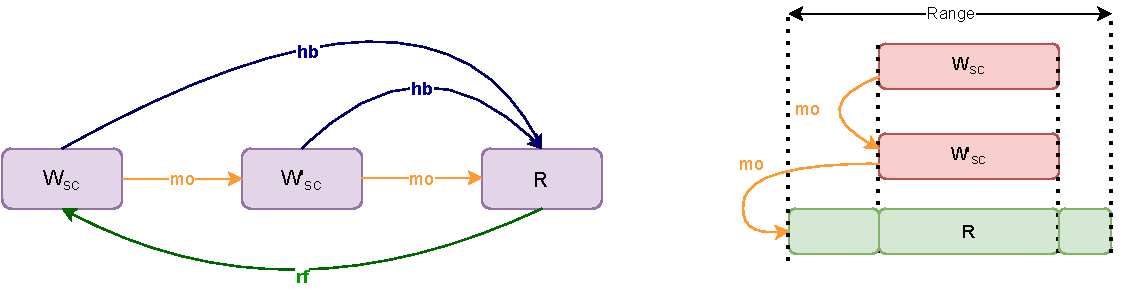
\includegraphics[scale=0.7]{4.ECMAScriptMemoryModel/SequentialAtomics2.pdf}
                        \caption{Second Axiom of SC-Atomics.}
                        \label{model:sc_atomics(2)}
                    \end{figure}
                
                \item If $g$ and $e$ are sequentially consistent, having equal ranges, and $d$ is bound to happen before them, then $e$ cannot read from $d$.
                    \begin{align*}
                        \et{g}{sc}\ \wedge\ \et{e}{sc}  
                        \ \wedge \ (\Re(g) \!= \!\Re(e)) 
                        \ \wedge \ \reln{d}{hb}{g} 
                        \ \wedge \ \reln{d}{hb}{e}
                        \ \Rightarrow \ 
                        \neg \ \reln{e}{rf}{d}.
                    \end{align*}

                    Figure~\ref{model:sc_atomics(3)} depicts pictorially the pattern that is not allowed by this rule.
                    \begin{figure}[H]
                        \centering 
                        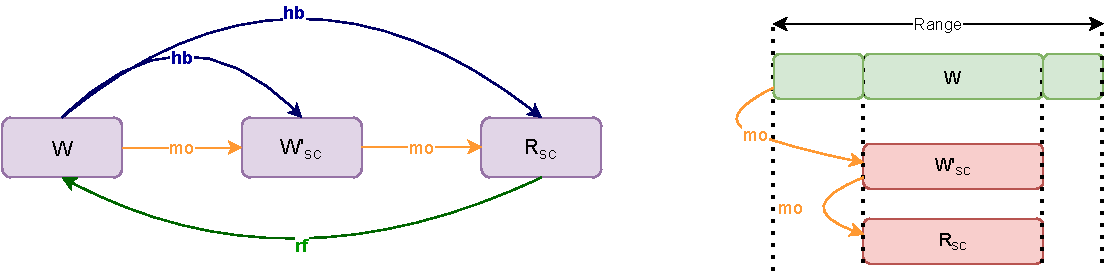
\includegraphics[scale=0.7]{4.ECMAScriptMemoryModel/SequentialAtomics3.pdf}
                        \caption{First Axiom of SC-Atomics.}
                        \label{model:sc_atomics(3)}
                    \end{figure}
                        
            \end{itemize}
        \end{axiom} 
        